In this chapter, we provide an evaluation proof of using IRS in kernel space. 
Experiments are setup for understanding the behavior of the six prototypes proposed in this thesis. 
Additionally, they are also used to provide a comparison with the user space implementation of IRS. 

\section{Setup}

The evaluation is performed with a virtual machine running on a hardware with maximum of 16 cores. 
The virtual machine can use from two to eight processor cores which is later used for the scaled up evaluation. 
The virtual machine is based on Intel Xeon E5-2650 - 2.00 GHz configured with Ubuntu 17.04 as the operating system. 
It is configured with 4GB RAM and 80GB hard disk. 
The virtual machine is configured with the LLVM-CLANG 3.9, GCC 4.9 and Boost 1.6.2.

\section*{Note}

We would be using the following abbreviations in the rest of the evaluations for simplicity of expression.
\begin{itemize}
\item {IRS\_Sh} - IRS user space implementation using shared scheduler design.
\item {IRS\_Opt} - IRS user space implementation using additional scheduler with conditional variable design.
\item {Proto\_1} - Prototype 1 discussed in the previous chapter.
\item {Proto\_2} - Prototype 2 discussed in the previous chapter.
\item {Proto\_3} - Prototype 3 discussed in the previous chapter.
\item {Proto\_4} - Prototype 4 discussed in the previous chapter.
\item {Proto\_5} - Prototype 5 discussed in the previous chapter.
\item {Proto\_6} - Prototype 6 discussed in the previous chapter.

\end{itemize}

\section{Evaluation Metrics}

\subsection{Execution Overhead}

Evaluation is done between the IRS user space solutions vs kernel space solutions. 
Execution overhead is calculated for each solution with respect to the plain execution of the bench-marking program. 
Unconstrained execution of the program is considered as plain execution. 

$$Execution Overhead = (T_{constr} - T_{plain})/T_{plain} * 100$$

$T_{constr}$ is the execution time of the bench-marking program when executed with the scheduling constraints. 
$T_{plain}$ is the plain execution time of the same bench-marking program. 
We expect to monitor the performance of various IRS implementations by checking this metric. 
If execution overhead for a certain IRS design is the smallest, that design is considered to give the best performance. 

\subsection{Number of valid synchronization calls} 

It is used to realize the number of voluntary calls made to kernel space for synchronization purposes. 
It is primarily the number of IOCTL calls made under the command - context\_switch, signal\_all\_other\_threads or set\_clock. 
We also find the number of voluntary context switch calls made to kernel space to determine the prototypes which can provide a smaller overhead. We observe the use of this metric more in this section~\ref{vol_kernel_calls}.


\section{Benchmarks}

We use four different bench-marking programs for the evaluation of this thesis. 
The bench-marking programs include:
\begin{itemize}
\item{Fibonacci} - Program runs with two threads computing Fibonacci numbers for 25 iterations per thread.
\item{Last Zero} - Program runs with 16 threads~\citep{abdulla2014optimal}.
\item{Indexer}- Program runs with 15 threads~\citep{dynamic_por}.
\item{Dining Philosophers Problem} - Program runs with 16 threads. 
This benchmark is motivated from the solution presented in \citet{silberschatz2014operating}.
\end{itemize}

\section{Voluntary kernel level calls \label{vol_kernel_calls}}

We evaluate the number of voluntary calls made to kernel space for synchronization. 
The evaluation is done across all six prototypes. 
The benchmark used for the evaluation is Fibonacci. 
The Fibonacci benchmark presents different levels of memory constraints via its traces. 
It has three traces providing 98 constraints, 44 constraints and 24 constraints respectively.

\begin{table}[h]
\begin{center}
 \begin{tabular}{|c c c|} 
 \hline
 & Prototype 1-4 & Prototype 5-6\\ %[0.5ex] 
 \hline
 Trace-1 & 300 & 175\\ 
 Trace-2 & 300 & 150\\
 Trace-3 & 300 & 150\\
 \hline
\end{tabular}
\end{center}
\caption{Number of IOCTL calls}
\label{num_ioctls}
\end{table}
\begin{table}
\begin{center}
 \begin{tabular}{|c c c|} 
 \hline
 & Prototype 1-4 & Prototype 5-6\\ %[0.5ex] 
 \hline
 Trace-1 & 150 & 27\\ 
 Trace-2 & 150 & 0\\
 Trace-3 & 150 & 0\\
 \hline
\end{tabular}
\end{center}
\caption{Number of context switch calls}
\label{num_ctxts}
\end{table}

From the tables~\ref{num_ioctls} and \ref{num_ctxts}, it is really evident that prototypes 5 and 6 reduce the number of calls made to kernel space. 
Prototypes 5 \& 6 are expected to provide better performance compared to other prototypes, when there are less dependencies between threads. 

Let us consider the Fibonacci benchmark, it has two threads with a total of 75 shared-memory events per thread. 
Thus, making a total of 150 memory events. 
For every shared-memory event, prototypes 1-4 trigger IOCTL calls to kernel space for context\_switch, signal\_all\_other\_threads or set\_clock. 
Therefore, having a total number of IOCTL calls as 300. 
In case of prototype 5-6, we have a proxy checking in user space which drastically reduces the calls to kernel space for additional synchronization. 
The set\_clock ioctl command is the only call made consistently for every memory access when using prototypes 5-6.

\begin{table}[h]
\begin{center}
 \begin{tabular}{|c c c c c c c|} 
 \hline
 & Proto-1 & Proto-2 & Proto-3 & Proto-4 & Proto-5 & Proto-6\\ %[0.5ex] 
 \hline
 Trace-1 & 406.833 & 454.785 & 385.416 & 455.745 & $277.793$ & $275.343$ \\ 
 Trace-2 & 367.199 & 520.352 & 352.506 & 509.843 & $160.266$ & $160.307$ \\
 Trace-3 & 351.029 & 416.653 & 333.704 & 412.206 & $152.425$ & $153.06$\\
 \hline
\end{tabular}
\end{center}
\caption{Execution overhead(\%) when compared with plain execution of Fibonacci}
\label{fib_exec_over}
\end{table}

Table~\ref{fib_exec_over} presents the reasoning of using prototypes 5-6. 
It shows the execution overhead is drastically reduced for the above mentioned prototypes. 
Reduction in the number of IOCTL calls makes a huge difference in the execution overhead. 
Prototypes 5-6 performs the best, when the following condition holds:
$num\_memory\_constraints << total\_memory\_events$.

\section{Scaled-up Evaluation}

In this evaluation, we understand the merits and demerits in the performance of the six prototypes and the two user space IRS implementations. 
For this evaluation, we use three bench-marking programs - last zero, indexer and dining philosophers problem. 
We scale the core count from two to eight processor cores and monitor the changes in the performance overhead across the three benchmarks for the various IRS implementations. 
For comparing the designs with IRS user space implementations, we have chosen the best prototype among the six for comparison. 

\subsection{Last Zero}

\citet{abdulla2014optimal} showcases this benchmark for the evaluation of their dynamic POR. 
The last zero program has 16 threads at its disposal. 
The pseudo code of this benchmark is depicted in listing~\ref{code_lastzero}. 
This benchmark is meant to provide memory constraints spread across different threads rather than being in two threads. 
The number of memory constraints provided in the trace files include: 15, 12, 5, 1 respectively. 
The maximum number of possible shared-memory events is 46.

\begin{figure}[h]
     \centering
     \subfloat[][User space vs Best Prototype]{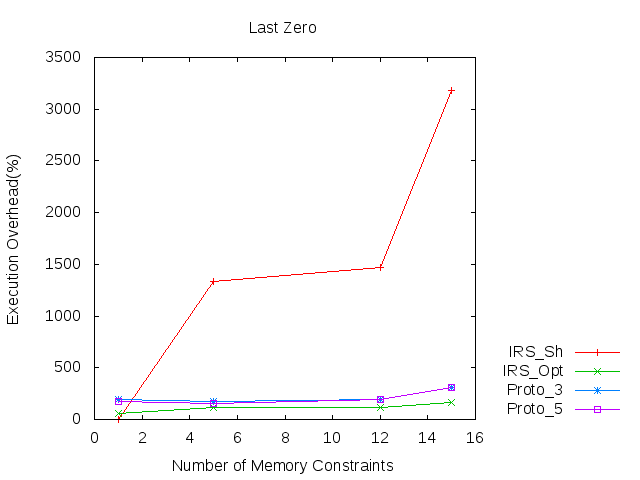
\includegraphics[scale=0.5]{../../evaluations/cores_2/eval_last_zero_best.png}\label{last_zero_best_cores_2}}
     \subfloat[][Comparison between prototypes]{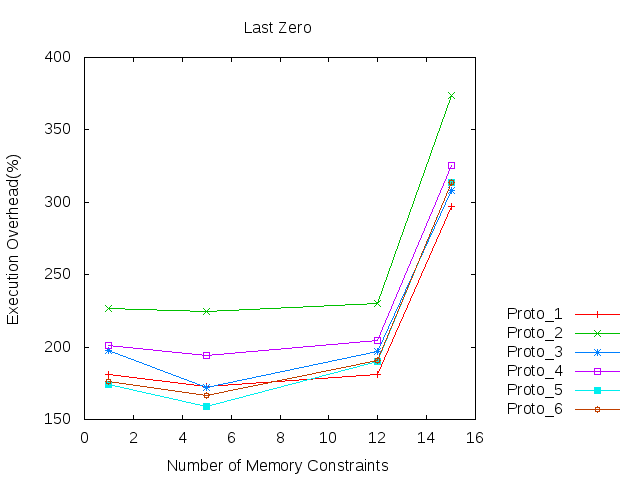
\includegraphics[scale=0.5]
{../../evaluations/cores_2/eval_last_zero_protos.png}
\label{last_zero_protos_cores_2}}
     \caption{Comparison of IRS with Last Zero on two cores}
\end{figure}


\begin{figure}[h]
     \centering
     \subfloat[][User space vs Best Prototype]{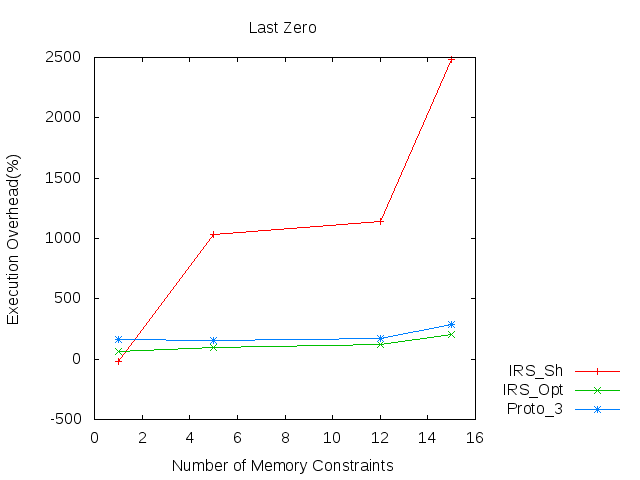
\includegraphics[scale=0.5]{../../evaluations/cores_4/eval_last_zero_best.png}\label{last_zero_best_cores_4}}
     \subfloat[][Comparison between prototypes]{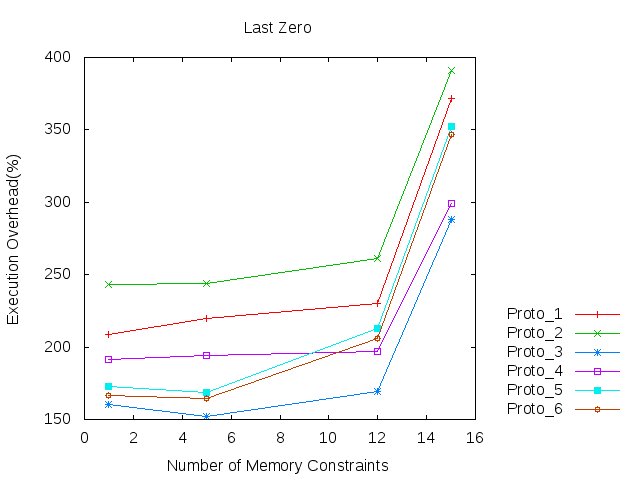
\includegraphics[scale=0.5]{../../evaluations/cores_4/eval_last_zero_protos.png}
\label{last_zero_protos_cores_4}}
     \caption{Comparison of IRS with Last Zero on four cores}
\end{figure}


\begin{figure}[h]
     \centering
     \subfloat[][User space vs Best Prototype]{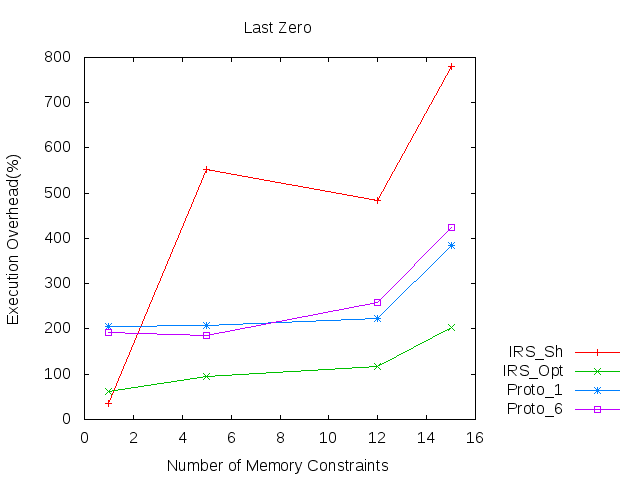
\includegraphics[scale=0.5]{../../evaluations/cores_8/eval_last_zero_best.png}\label{last_zero_best_cores_8}}
     \subfloat[][Comparison between prototypes]{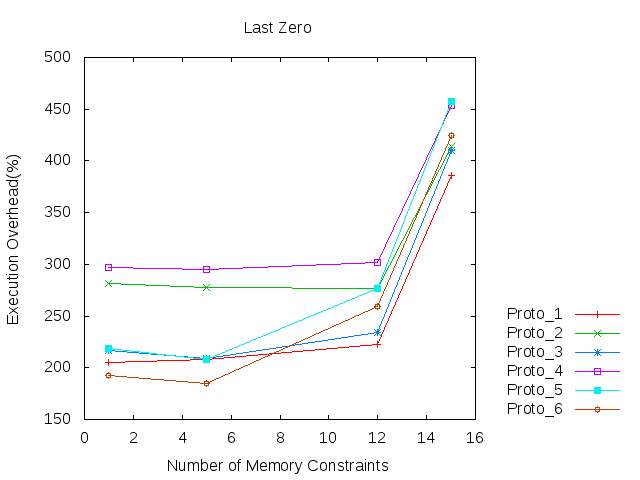
\includegraphics[scale=0.5]{../../evaluations/cores_8/eval_last_zero_protos.png}
\label{last_zero_protos_cores_8}}
     \caption{Comparison of IRS with Last Zero on eight cores}
\end{figure}

The benchmark has 16 threads and the memory constraints are spread across threads. 
Thus, making it expensive in regard to execution time. 
IRS\_Sh is expected to be the worst of all designs considering the fact that it is a busy waiting design. 
Busy waiting design makes the waiting thread to constantly poll one of the cores thus, making it performance inefficient. 
However, it is expected to improve the execution overhead with the scaling of cores. 
IRS\_Opt is designed using conditional variables and it is expected to perform better than IRS\_Sh for scaled evaluations.
IRS\_Opt is expected to provide a better performance among all the designs because the $num\_memory\_constraints << total\_memory\_events$. 
Proto\_5 and Proto\_6 are also expected to provide better results with this benchmark, since the above condition holds good for these prototypes.

From Fig~\ref{last_zero_protos_cores_2}, it is evident that Proto\_5 and Proto\_6 performs nearly the same when it comes to execution overhead. 
Surprisingly, Proto\_3 performs better in these evaluations because they are expected to provide good performance when the number of memory constraints are higher in the bench-marking program. 
It is nearly true in case of evaluations with four cores and eight cores from Fig~\ref{last_zero_protos_cores_4} and Fig~\ref{last_zero_protos_cores_8}. 
From Figures~\{\ref{last_zero_best_cores_2}, \ref{last_zero_best_cores_4}, \ref{last_zero_best_cores_8}\}, it is evident that IRS\_Sh is the worst implementation for this benchmark among all the other implementations. 
From the above figures, the validity of improvement in execution overhead with scaling cores for IRS\_Sh holds. 




%----------------------------------------------------------------------------
\subsection{Indexer}



%Evaluation of indexer with cores-------
\begin{figure}[h]
     \centering
     \subfloat[][User space vs Best Prototype]{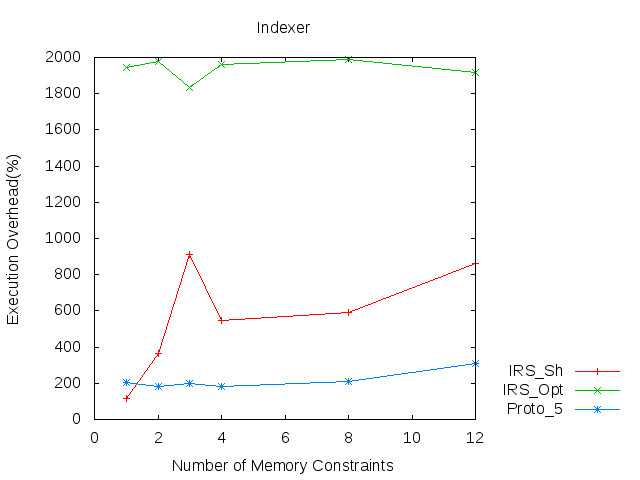
\includegraphics[scale=0.5]{../../evaluations/cores_2/eval_indexer_best.png}\label{indexer_best_cores_2}}
     \subfloat[][Comparison between prototypes]{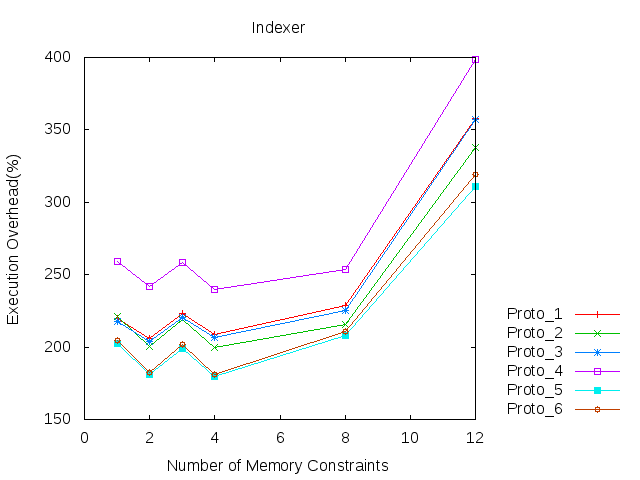
\includegraphics[scale=0.5]{../../evaluations/cores_2/eval_indexer_protos.png}\label{indexer_protos_cores_2}}
     \caption{Comparison of IRS with Indexer on two cores}
\end{figure}


\begin{figure}[h]
     \centering
     \subfloat[][User space vs Best Prototype]{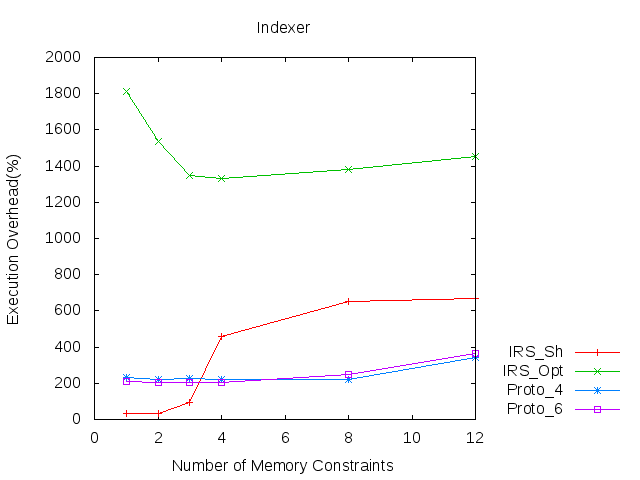
\includegraphics[scale=0.5]{../../evaluations/cores_4/eval_indexer_best.png}\label{indexer_best_cores_4}}
     \subfloat[][Comparison between prototypes]{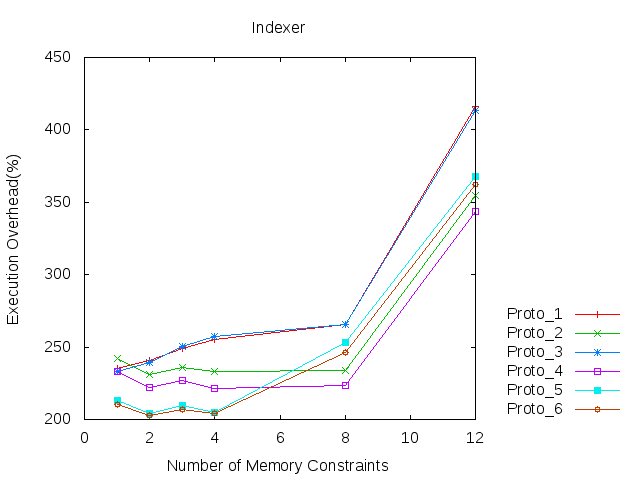
\includegraphics[scale=0.5]{../../evaluations/cores_4/eval_indexer_protos.png}\label{indexer_protos_cores_4}}
     \caption{Comparison of IRS with Indexer on four cores}
\end{figure}


\begin{figure}[h]
     \centering
     \subfloat[][User space vs Best Prototype]{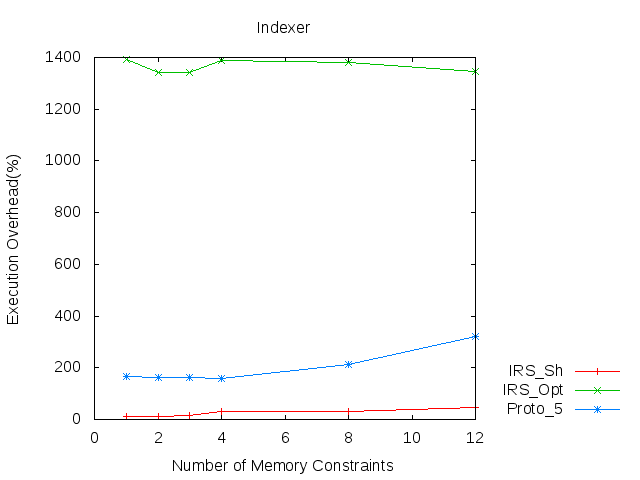
\includegraphics[scale=0.5]{../../evaluations/cores_8/eval_indexer_best.png}\label{indexer_best_cores_8}}
     \subfloat[][Comparison between prototypes]{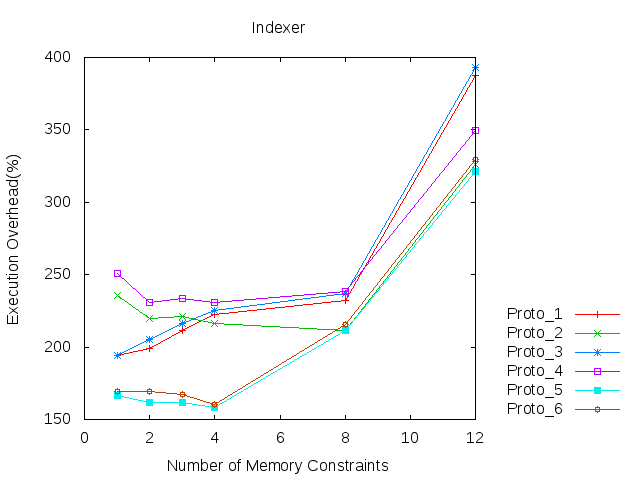
\includegraphics[scale=0.5]{../../evaluations/cores_8/eval_indexer_protos.png}\label{indexer_protos_cores_8}}
     \caption{Comparison of IRS with Indexer on eight cores}
\end{figure}

\citet{dynamic_por} utilizes this benchmark for evaluating their dynamic POR design. 
The pseudo code for the indexer program is realized in listing~\ref{code_indexer}.  
The indexer program revolves around a hash table, where threads read and write hashed messages on it. 
Each thread calculates four messages and writes them to a shared hash table. 
Collision are detected and avoided using compare and swap statement. 
The message values depend on the thread id. 

For our experiments, we have used 15 threads with the indexer program. 
The benchmark contains approximately 60 shared-memory events in total. 
Six traces are used with the following as the number of memory constraints: 12, 8, 4, 3, 2, 1. 
The memory constraints are set in a way that most of the constraints are within a span of few threads and not all 15 threads. 
We expect to have good performance for IRS\_Sh because the number of constraints are not spread across all 15 threads. 
We expect it to perform the best when the core count is 8, even when the constraints are set at 12. 
Proto\_5 and Proto\_6 are expected perform better for this benchmark, since the condition $num\_memory\_constraints << total\_memory\_events$ holds. 

From Figs~\{\ref{indexer_protos_cores_2}, \ref{indexer_protos_cores_4}, \ref{indexer_protos_cores_8}\}, it is evident that Proto\_5 and Proto\_6 performs the best in almost all scenarios. 
Thus, maintaining the above condition. 
Based on the analysis of Figs~\{\ref{indexer_best_cores_2}, \ref{indexer_best_cores_4}, \ref{indexer_best_cores_8}\}, we observe a trend in the improvement of execution overhead in IRS\_Sh. 
As expected IRS\_Sh seems to give the best performance when the number of cores is eight as observed in Figure~\ref{indexer_best_cores_8}.
IRS\_Opt showcases a huge overhead for this benchmark, because of the lack of diversity in the memory constraints(spread of memory constraints across all threads). 


%----------------------------------------------------------------------------
\subsection{Dining Philosopher's Problem}

%Evaluation of Dining Phil with cores-------
\begin{figure}[h]
     \centering
     \subfloat[][User space vs Best Prototype]{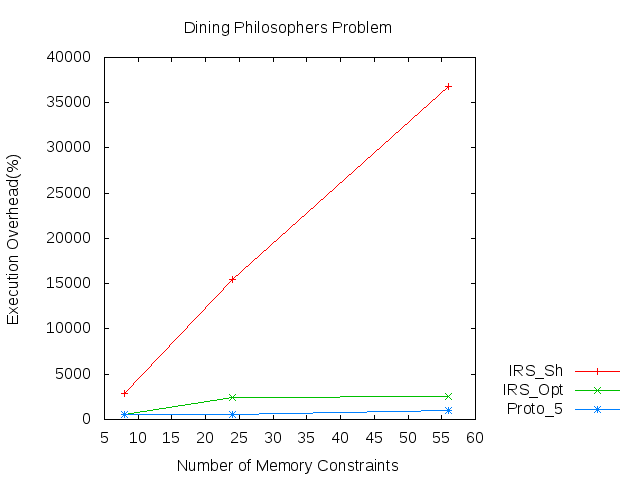
\includegraphics[scale=0.5]{../../evaluations/cores_2/eval_dining_phil_best.png}\label{dining_phil_best_cores_2}}
     \subfloat[][Comparison between prototypes]{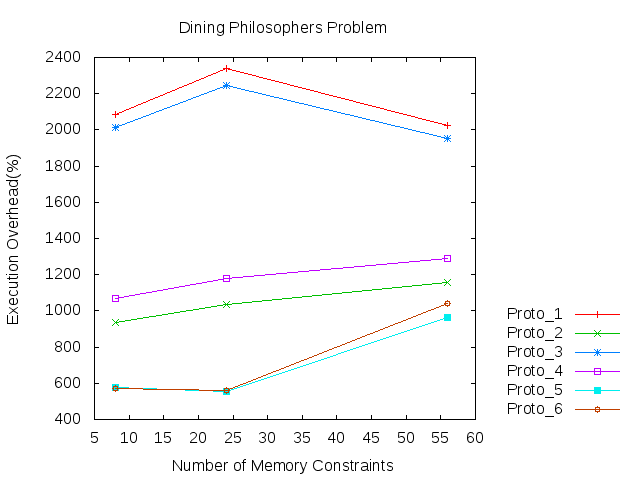
\includegraphics[scale=0.5]{../../evaluations/cores_2/eval_dining_phil_protos.png}\label{dining_phil_protos_cores_2}}
     \caption{Comparison of IRS with Dining Philosophers Problem on two cores}
\end{figure}

\begin{figure}[h]
     \centering
     \subfloat[][User space vs Best Prototype]{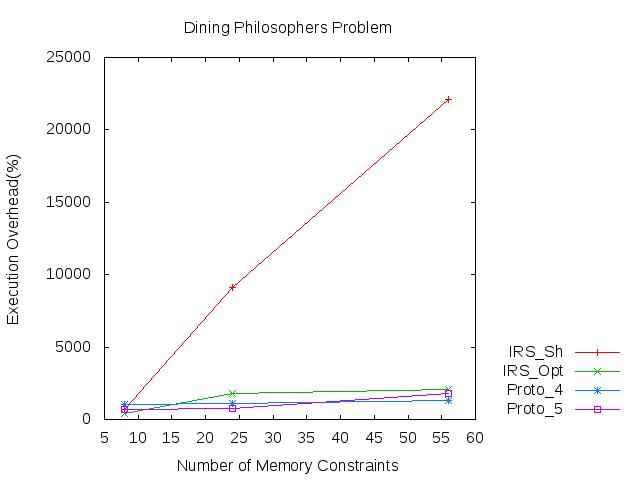
\includegraphics[scale=0.5]{../../evaluations/cores_4/eval_dining_phil_best.png}\label{dining_phil_best_cores_4}}
     \subfloat[][Comparison between prototypes]{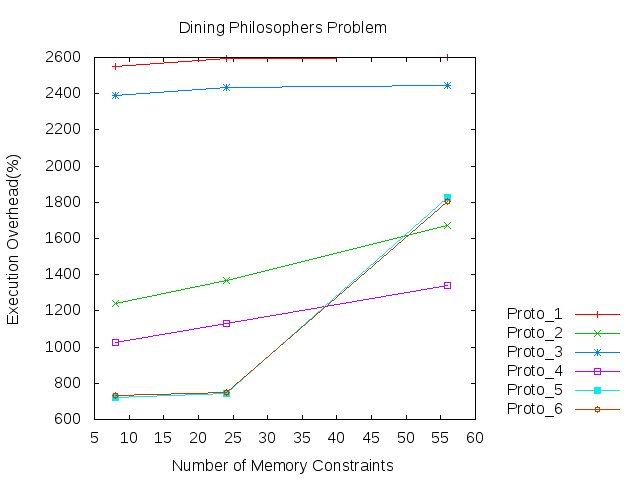
\includegraphics[scale=0.5]{../../evaluations/cores_4/eval_dining_phil_protos.png}\label{dining_phil_protos_cores_4}}
     \caption{Comparison of IRS with Dining Philosophers Problem on four cores}
\end{figure}

\begin{figure}[h]
     \centering
     \subfloat[][User space vs Best Prototype]{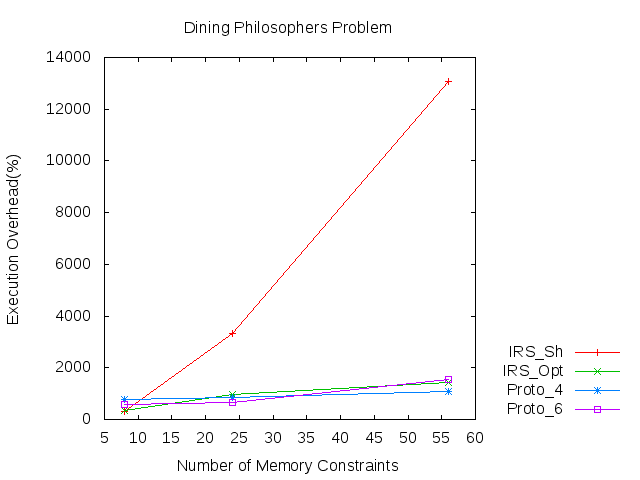
\includegraphics[scale=0.5]{../../evaluations/cores_8/eval_dining_phil_best.png}\label{dining_phil_best_cores_8}}
     \subfloat[][Comparison between prototypes]{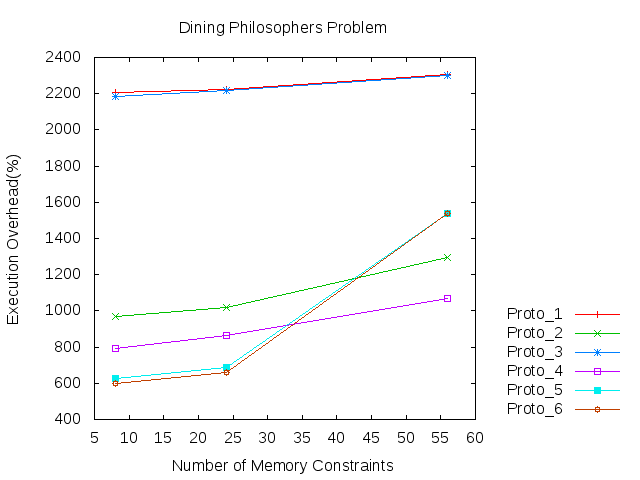
\includegraphics[scale=0.5]{../../evaluations/cores_8/eval_dining_phil_protos.png}\label{dining_phil_protos_cores_8}}
     \caption{Comparison of IRS with Dining Philosophers Problem on eight cores}
\end{figure}

Dining Philosopher's Problem is a well known synchronization problem in the domain of concurrency problems. 
There are many solutions adhered to overcome the problem. 
\citet{silberschatz2014operating} have addressed many solutions in their book for the above problem. 
We are using one of the solutions proposed in their book. 
The solution uses two classes of philosophers - odd and even philosopher. 
The classification is based on their thread id. 
Every odd philosopher checks the chopstick on the left before checking on the right for availability. 
The opposite in case of even philosopher. 
The solution for this problem is showcased in listing~\ref{code_dining_phil}.

In our experiments, we have adapted the solution to have 16 threads and number of iterations as 10. 
Compared to previous benchmarks which had only few number of constraints. 
This benchmark has more constraints spread across all 16 threads. 
This benchmark is expected to run in milliseconds time range rather than microseconds which was evident with respect to the previous benchmarks. 
For getting a detailed understanding of the experimental results, please refer to appendix~\ref{appendixb}.  

There are nearly 60 shared-memory events per thread. 
Thus, making a total of 960 shared-memory events in total. 
The benchmark has at-most eight threads running at any point of time. 
The number of memory constraints listed for the three traces include: 56, 24, 8.
The number of memory constraints is too small compared to the total number of shared memory events in the bench-marking program. 
Proto\_1 and Proto\_3 are kernel space solutions implemented with a shared scheduler in place. 
Because of constant kernel synchronization calls during shared-memory events, Proto 1-4 are expected to provide a high overhead. 
However, the Proto\_2 and Proto\_4 uses a separate thread for scheduling, the IOCTL call made from $AfterMA()$ only increments the vector clock. 
Whereas in case of Proto\_1 and Proto\_3, we have calls made from $AfterMA()$ which performs signalling of other threads. Signalling of other threads is a costly operation compared to updating a vector clock. 
Thus, making Proto\_1 and Proto\_3 to perform the worst among the prototypes. 
The condition $num\_memory\_constraints << total\_memory\_events$ holds for this benchmark, we expect the Proto\_5 and Proto\_6 to provide the best performance among the prototypes.
IRS\_Opt is expected to have a good performance since the above condition holds true for the design.
IRS\_Sh is expected to give away a very poor performance because of the diversity of constraints.  

From Figs~\{\ref{dining_phil_protos_cores_2}, \ref{dining_phil_protos_cores_4}, \ref{dining_phil_protos_cores_8}\}, it is evident that Proto\_5 and Proto\_6 performs the best in all the scenarios. 
Proto\_1 and Proto\_3 as expected came up with the worst performance among the prototypes. 
In case of the comparison with the user space implementation, IRS\_Opt seems have smaller overhead compared to IRS\_Sh. 
From Figs~\{\ref{dining_phil_best_cores_2}, \ref{dining_phil_best_cores_4}, \ref{dining_phil_best_cores_8}\}, it is evident that IRS\_Sh seems to give away the worst performance for this benchmark because of its busy waiting design. 


\section{Summary}

The Fibonacci bench-mark helped us in understanding the behavior of prototypes. 
The scaled up experiments clearly explained the merits and demerits of various IRS designs. 
The scaled up experiments show that Proto\_5 and Proto\_6 seem to perform the best among the prototypes in nearly all the scenarios given in the bench-marking programs. 
IRS\_Sh implementation seems to give away the worst performance in nearly all benchmarks. 
From the experiments, it is evident that Prototypes 1-4 suffer from the problem of scalability. 
The performance of user space implementation overshadows the kernel space implementation when the number of memory constraints are in single digits. 
 
By observing the above results we can conclude that we need to have a solution which is combination of IRS\_Opt and Prototypes 5-6. 
This implementation would have a loadable kernel module similar to Proto\_5 and Proto\_6 however, without any checking for memory permissions in kernel space for the threads. 
The kernel module would help in providing as a forced yield of processor to the OS Scheduler from the thread and also an interface to revive the thread. 
The check for memory permission would be implemented entirely in user space and calls would be made to the above mentioned kernel space solution for yielding the processor.  
In short this kernel space interface would be used instead of using a condition variables in IRS\_Opt.
